\section{Management von Betriebsdaten im Industriebetrieb}\label{sec:usecase}
Die Aufgaben eines Industriebetriebs sind in erster Linie die Entwicklung und Herstellung neuer marktfähiger Produkte. 
Im Rahmen von industriellen Betrieben, die einer ständigen Dynamik des Wettbewerbs durch sich verändernde Marktbedingungen ausgesetzt sind, liegt der Fokus letztlich auf der Steigerung der Effizienz, also die Verbesserung von Durchlaufzeiten, Qualität und Auslastung in der Fertigung.
\cite{Erlach.2010}
Demnach muss ein Unternehmen nach Agilität und Effizienz ihrer Geschäftsprozesse streben, um auf diese Evolution angemessen reagieren und die sich daraus ergebenden Chancen aktiv ergreifen zu können.
 In zunehmendem Maße werden deshalb Anwendungen und Maschinenanlagen für \ac{IT}-gestützte und flexibel automatisierbare Produktionsabläufe eingesetzt. 
\cite{Erlach.2010}

Die Betriebswirtschaftslehre bezeichnet in diesem Kontext alle Komponenten, die in den betrieblichen Geschäftsprozessen zur Leistungserstellung miteinander kombiniert werden, als Produktionsfaktoren. 
Traditionell wird die Arbeit dabei unterteilt in dispositive und ausführende Arbeit. Die anderen Produktionsfaktoren stellen Betriebsmittel, Anlagen und Kapital dar.
\cite{Kanel.2018}
Informationen bilden die Grundlage bei stategischen sowie operativen Entscheidungen im Unternehmen und stellen damit einen wesentlichen Produktionsfaktor im betrieblichen Leistungserstellungsprozess dar.
\cite{Scheer.1990}
Die rechtzeitige Bereitstellung von Informationen sowie die Möglichkeit der unmittelbaren und dynamischen Informationsverarbeitung sind zu einem kritischen Erfolgsfaktor von Unternehemen geworden. 
Um dies gewährleisten zu können, ist ein professionelles Management der Betriebsdaten im Industriebetrieb erforderlich.
\cite{Dippold.2005}
Industriellen Betrieben mangelt es jedoch häufig an Transparenz in den wertschöpfenden Geschäftsprozessen.
Eine zeitnahe Rückkopplung zwischen den vom Management gesetzten Zielen und der tatsächlich erreichten Leistung bei der Abwicklung wertschöpfender Geschäftsprozesse findet oftmals nur unzureichend statt. 
\cite{Grauer.2019}

Die Vision einer ganzheitlichen und transparenten Betrachtung der betrieblichen Geschäftsprozesse zur Leistungserstellung führte in den Siebzigerjahren zu den Anfängen der computerintegrierten Fertigung, englisch \textit{\acf{CIM}}. 
Mit der zunehmenden Durchdringung von Industriebetrieben mit \ac{IT}-Systemen, erregte das Modell der computerintegrierten Fertigung anschließend weltweit Aufsehen und etablierte die durchgängig \ac{IT}-gestützte Betriebsdatenerfassung der betriebswirtschaftlichen und technische Aufgaben eines Industriebetriebs auf Basis einer bereichsübergreifenden Datenbasis.
\cite{Scheer.1990}

Um den unterschiedlichen Auffassungen über \ac{CIM} eine gemeinsame Definition zu verleihen, sprach der \citeauthor{AusschufurWirtschaftlicheFertigung.1985} im Jahre \citeyear{AusschufurWirtschaftlicheFertigung.1985} eine Empfehlung aus, ihn als integrierten \ac{IT}-Einsatz in allen mit der Produktion zusammengehörenden Bereichen eines Industriebetriebs zu verstehen. 
Eine Integration der technischen und betriebswirtschaftlichen Aufgaben innerhalb der Produktherstellung soll durch die Nutzung einer gemeinsamen Datenbasis erreicht werden. 
Das \ac{CIM}-Konzept umfasst die Anwendungen des Computer-aided Designs, des Computer-aided Plannings, des Computer-aided Manufacturings , der Computer-aided Quality Assurance und der \ac{PPS}.
\cite{AusschufurWirtschaftlicheFertigung.1985}

Im Zuge der Einführung eines \ac{PPS}-Systems, wird der reine Planungsaspekt jetzt durch Steuerungsfunktionalitäten ergänzt. Ein Beispiel stellt die Erfassung von Rückmeldedaten aus den Produktionsbereichen dar, wodurch gezielte Eingriffe zur Optimierung der Geschäftsprozesse durch transparente Zwischenstände in der Fertigung ermöglicht werden.
\cite{Dickersbach.2014}
Die \ac{PPS} sowie viele weitere Kernfunktionen eines Industriebetriebs lassen sich heute unter dem Begriff \textit{\acf{ERP}} subsumieren. Im Gegensatz zu \ac{CIM} geht die Vision eines \ac{ERP}-Systems noch einen Schritt weiter und unterstützt auf Basis einer gemeinsamen Datenbasis ganzheitlich alle betriebswirtschaftlichen Geschäftsprozesses eines Unternehmens.
Insofern entsteht Transparenz über die gesamten betrieblichen Geschäftsprozesse eines Unternehmens von der strategischen Planung bis zur Qualitätssicherung.
\cite{Leiting.2012}

Der Fokus der folgenden Betrachtungen dieser Bachelorarbeit liegt insbesondere auf dem Modul \ac{PPS} der \ac{ERP}-Lösung \textit{S/4HANA Cloud} von SAP, die als Nachfolger der verbreiteten \textit{SAP Business Suite} gilt. 
\cite{Densborn.2018}
Die Komponente \ac{PPS} ist seit der Einführung der \ac{ERP}-Lösung \textit{SAP R/2} im Jahre 1983 ein Bestandteil der SAP \ac{ERP}-Lösungen und wurde seit dem ständig weiterentwickelt.
\cite{Frick.2008}

\subsection{Geschäftsprozesse in der Produktionsplanung und -steuerung}
Die Aufgabenberieche für die \ac{PPS} sind innerhalb von SAP S/4HANA Cloud, wie auch bei seinen Vorgängern, im Modul PP angeordnet. Die wesentlichen Geschäftsprozesse innerhalb von PP sind die Absatz- und Produktionsgrobplanung, die Programmplanung, die Materialbedarfsplanung, die Langfristplanung, die Fertigungsauftragseröffnung und -durchführung sowie die Kapazitätsplanung. 
\cite{Akhtar.2019} 

Im Wesentlichen umfassen diese Geschäftsprozesse in der Produktionsplanung und -steuerung die folgenden Bereiche:

\begin{itemize}
    \item 
    \textbf{Absatz- und Produktionsgrobplanung} zur Bestimmung der herzustellenden Mengen
    \item 
    \textbf{Materialbedarfsplanung} zur Bestimmung der Bedarfe unter Einbeziehung von Ausschuss und Losgrößen
    \item 
    \textbf{Kapazitätsplanung} zur Feinplanung unter Einbeziehung der Produktionskapazitäten
    \item 
    \textbf{Fertigungssteuerung} zur Steuerung und Erfassung der Fertigungsdurchführung
\end{itemize}

Diese vier Bereiche stellen den Prozessumfang jedoch nur sehr grob dar, weshalb Abbildung \ref{fig:Prozessüberblick der Produktionsplanung und -steuerung} einen detaillierteren Überblick geben soll. Hier sind die relevanten Geschäftsprozesse explizit mit ihren wichtigsten Eingangs- und Ausgangsgrößen dargestellt.

Die Produktionsplanung umfasst sowohl die Absatz- als auch die Produktionsgrobplanung. Zukünftige Bedarfe werden in der Absatzplanung geplant. Dabei spielen weder Bestände noch Kapazitätsangebote eine Rolle. Die Verkaufshistorie stellt oft die Grundlage für die Absatzplanung dar. Basierend auf der Absatzplanung ermittelt die Produktionsgrobplanung nun die geplanten Produktionsmengen. Anfangsbestände und Kapazitäten können grob berücksichtigt werden. Die Programmplanung führt die Absatzplanung mit den Bedarfen aus Kundenaufträgen zusammen und ermittelt auf diese Weise die Primärbedarfe für die Produktion. 
\cite{Dickersbach.2014} 

\begin{figure}[H]
	\centering 
    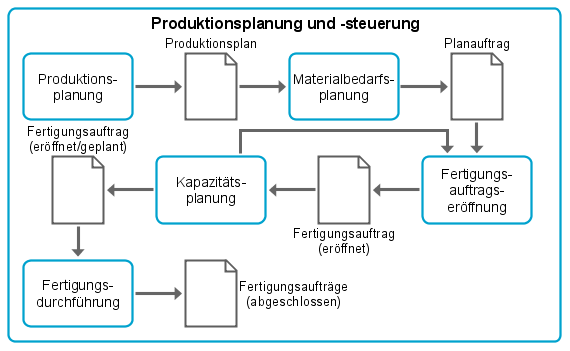
\includegraphics[width=\textwidth]{img/Produktion.png}	
    \caption[Prozessüberblick der Produktionsplanung und -steuerung]
    {Produktionsplanung und -steuerung in SAP S/4HANA Cloud\protect\footnotemark}
    \label{fig:Prozessüberblick der Produktionsplanung und -steuerung}
\end{figure}
\footnotetext{Eigene Darstellung, in Anlehnung an \citeauthor{Akhtar.2019} \citeyear{Akhtar.2019} \cite{Akhtar.2019} }
\footnotetext{Die Abbildung dient lediglich der Visualisierung und ist nicht \ac{BPMN} 2.0 konform.}

Die Materialbedarfsplanung berechnet auf Basis des Produktionsplans für alle Ebenen die Bedarfsdeckung. Berücksichtigt werden unter anderem Durchlaufzeiten, Losgrößen und Ausschußmengen.
In der Kapazitätsplanung wird der Arbeitsvorrat aus den Vorgängen eröffneter oder freigegebener Fertigungsaufträge eingeplant. Das Ergebnis der Kapazitätsplanung ist eine realisierbare Auftragsabfolge für die Fertigung.
\cite{Dickersbach.2014} 

Das zentrale Geschäftsobjekt für die Steuerung und Erfassung der Fertigung ist der Fertigungsauftrag. Die Fertigungsauftragseröffnung beschreibt die Erstellung des Fertigungsauftrags. 
Während sich die vorhergehenden Prozesse mit der Produktionsplanung befassen, beschäftigt sich die Fertigungsdurchführung mit der Erfassung und Steuerung der Ist-Situation der Fertigung im Fertigungsauftrag.
\cite{Dickersbach.2014} 

Die zugrunde liegenden Stammdaten der Produktionsplanung und -steuerung in SAP S/4HANA Cloud sind der Materialstamm, die Stückliste, der Arbeitsplan und der Arbeitsplatz. 
\cite{Dickersbach.2014}

\subsection{Vorstellung der Fertigungsdurchführung in der diskreten Fertigung}
In der Terminologie der SAP \ac{ERP}-Lösungen wird die Fertigung in die Fertigungsarten diskrete Fertigung, Serienfertigung, Prozessfertigung, Kanban und Projektfertigung eingeteilt. 

Die diskrete Fertigung\footnotetext{In anderer Literatur wird die \textit{diskrete Fertigung} auch als \textit{Werkstattfertigung bezeichnet.}} befasst sich mit der Herstellung von Produkten basierend auf Fertigungsaufträgen. 
Die diskrete Fertigung ist dann erforderlich, wenn die Herstellung von Erzeugnissen in einer variantenreichen Ausprägung benötigt wird, wenn die Auftragslage sehr unregelmäßig ist und die Fertigung anhand von Arbeitsplätzen abläuft. 
\cite{Mathieu.2014}
Des Weiteren lässt sich die diskrete Fertigung im SAP-Standard auf verschiedene Wege durchführen. Auf der einen Seite gibt es die Lagerfertigung, bei der die gesamte Planung, unabhängig von Kundenaufträgen, auf Basis der Planprimärbedarfe erfolgt. Im Gegenzug dazu existiert die Kundeneinzelfertigung bei der ein Fertigungsauftrag erst mit Eingang eines expliziten Kundenauftrags erstellt wird. Eine umfassende Erörterung der anderen Fertigungsarten und Planungsstrategien ist in dieser Bachelorarbeit nicht angedacht, kann aber der verwendeten Literatur entnommen werden.
\cite{Dickersbach.2014}

Der Produktionsprozess in der diskreten Fertigung beginnt, wenn ein Fertigungsauftrag erstellt wird. 
Ein Fertigungsauftrag kann entweder manuell oder durch die Umwandlung eines Planauftrags, die das System nach der Ausführung der Bedarfsplanung erzeugt hat, erstellt werden. 
Ein Fertigungsauftrag gibt an welches Produkt zu welchem bestimmten Zeitpunkt zu welcher Gutmenge zu produzieren ist. 
Er legt ebenfalls die Arbeitsplätze und Materialien, die für die Fertigung benötigt werden, fest. 
\cite{Dickersbach.2014}

Fertigungsaufträge werden am Tag der geplanten Freigabe, sofern die erforderlichen Materialien und Kapazitäten verfügbar sind, erteilt. 
Dokumente, die sich auf den Fertigungsauftrag beziehen, werden gedruckt, um die Fertigungsdurchführung vorzubereiten. 
Die zur Herstellung der Produkte erforderlichen Materialien werden anhand des Fertigungsauftrags entnommen, das Produkt anhand des Fertigungsauftrags hergestellt und die angefallenen Mengen \textit{(Gutmenge, Ausschuss, Nacharbeit)} werden anhand des Fertigungsauftrags zurückgemeldet.
Das Produkt wird eingelagert und der Wareneingang gebucht. 
Zur Minimierung des Aufwands während der Betriebsdatenerfassung kann der Wareneingang mithilfe der Rückmeldung des Auftrags in SAP S/4HANA Cloud automatisch gebucht werden.
Die Abwicklung des Fertigungsauftrags ist anschließend sicherzustellen, woraufhin der Fertigungsauftrag als abgeschlossen deklariert wird und nicht mehr änderbar ist.
\cite{Dickersbach.2014}

\begin{figure}[H]
	\centering 
    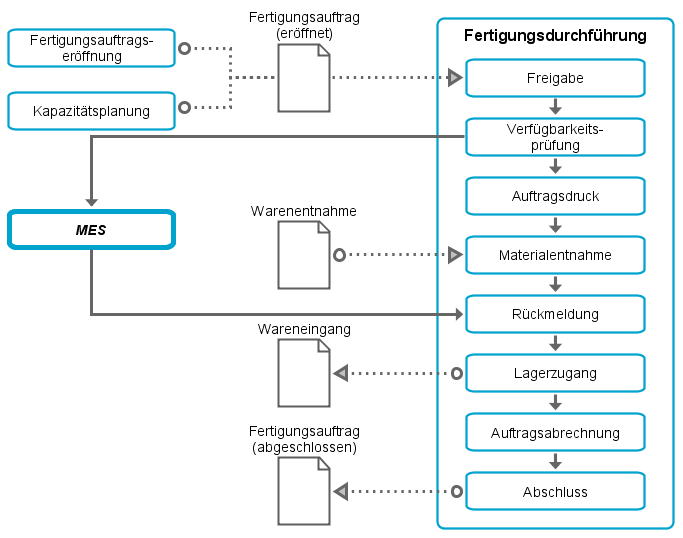
\includegraphics[width=\textwidth]{img/fertigungsdurch_ist.png}	
    \caption[Überblick über die Prozesse der diskreten Fertigung]
    {Überblick über die Prozesse der diskreten Fertigung\protect\footnotemark}
    \label{fig:Überblick über die Prozesse der diskreten Fertigung}
\end{figure}
\footnotetext{Eigene Darstellung, in Anlehnung an \citeauthor{Dickersbach.2014} \citeyear{Dickersbach.2014} \cite{Dickersbach.2014} }
\footnotetext{Die Abbildung dient lediglich der Visualisierung und ist nicht \ac{BPMN} 2.0 konform.}

Der Fertigungsauftrag verfolgt die Zwecke, sowohl der Fertigungslenkungung als Schaffung der benötigen Transparenz bezüglich mengen- und kostenmäßigen Kennzahlen in der Fertigung. Zur Steuerung der Fertigung gehört unter anderem die Bereitstellung der für die Fertigung notwendigen Informationen über die auszuführenden Vorgänge. Hierzu wird es benötigt, dass der Fertigungsauftrag Stammdaten und Betriebsdaten behandelt. Basierend auf dem Arbeitsplan und der Stückliste lässt sich der Fertigungsauftrag im Wesentlichen auf folgende Daten unterteilen:

\begin{itemize}
    \item \textbf{Kopfdaten} die den organisatorischen Rahmen formalisieren. Hierzu zählen die Auftragsnummer, die Kosten sowie die Terminierung des Auftrags
    \item \textbf{Vorgangsdaten} die neben den Details zu den durchzuführenden Vorgängen auch die Rückmeldungen aus der Fertigung sowie die geplanten Durchführungstermine enthalten
    \item \textbf{Komponentendaten} die den Bedarf an Materialien sowie deren Reservierungsinformationen angeben.
\end{itemize}

Im Rahmen der Betriebsdatenerfassung werden die realisierten Mengen- und Zeitwerte der Fertigungsaufträge und Mitarbeiter, Warte- und Ausfallzeiten von Betriebsmitteln sowie der Einsatz von Materialien in SAP S/4HANA Cloud zurückgemeldet. Insbesondere ein unmittelbarer Eingriff in die diskete Fertigung benötigt die Informationen über den Zustand des Produktionsprozesses in Echtzeit. 

Die SAP \ac{ERP}-Lösungen sehen dabei diverse Rollen für die Durchführung der Fertigung vor. In der Praxis hat sich jedoch gezeigt, dass diese oftmals vom Standard abweichen, da die Befugnisse der Fertigungsmitarbeiter stark an unternehmensspezifische Richtlinien gekoppelt sind.
\cite{Frick.2008}
In SAP S/4HANA Cloud werden für die Fertigungsdurchführung standardmäßig die folgenden zwei Rollen vorgesehen:
\begin{itemize}
    \item \textbf{Fertigungssteuerer}: Der Fertigungssteuerer ist laut dem Rollenkonzept der SAP verantwortlich für die Freigabe eines Fertigungsauftrags. Zudem liegt es in seinem Zuständigkeitsbereich auf veränderte Situationen in der Fertigungsdurchführung zu reagieren und unmittelbar kurzfristige Planungsentscheidungen zu treffen.
    \item \textbf{Werker}: Der Werker hat Fertigungsaufträge und Vorgänge nach Anweisung auszuführen. Er steht in der Pflicht möglicht unmittelbar, aber zwingend fristgerecht Rückmeldungen bezüglich der Fortschritte zu erfassen.
\end{itemize}

Eine Alternative, die als Vorgehensweise ebenfalls eine weite Verbreitung gefunden hat, ist es die erstellten und freigegebenen Fertigungsaufträge an ein sogenanntes \ac{MES} weiterzugeben, dort die eigentliche Fertigungssteuerung sowie die Kapazitätsplanung vorzunehmen und die Rückmeldungen der Fertigungsaufträge über Schnittstellen an SAP S/4HANA Cloud weiterzugeben. 
\cite{Gerberich.2011}
In diesem Fall wird der Funktionsumfang der \ac{PPS} von SAP S/4HANA Cloud  für die Materialbedarfsplanung, für die Bestandsrechnung und für die Kostenabrechnung verwendet.
\cite{Dickersbach.2014}
Das Konzept eines \ac{MES} wird in dieser Bachelorarbeit nicht weiter vertieft, daher sei lediglich auf weiterführende Literatur verwiesen.
\cite{Kletti.2007} \cite{Gerberich.2011}


Das Prinzip der diskreten Fertigung stellt den Werker in den Mittelpunkt der Wertschöpfung. 
Er verarbeitet die Materialien an einem Arbeitsplatz, falls nötig mit der Unterstützung von Maschinen und erzeugt das Endprodukt. 
\cite{Gerberich.2011}
Da die diskrete Fertigung zumeist in Form einer Kundeneinzelfertigung angewendet wird, sind niedrige bis mittlere Gutmengen und eine hohe Produktvarianz die Regel. 
Eine weitere Eigenschaft der diskreten Fertigung ist bedingt durch die erwähnte Produktvarianz. Diese macht es notwendig die Produktion flexibel planen zu können, da meist mehrere Vorgänge zur Herstellung eines Produktes von Nöten sind.
Dabei werden Transporte von Arbeitsplatz zu Arbeitsplatz zum Normalfall.
Eine vollautomatische Betriebsdatenerfassung und -verarbeitung ist in der Praxis daher beinahe ausgeschlossen.
Die Betriebsdatenerfassung wird in der Regel manuell über sogenannte \ac{MES}-Terminals vorgenommen.
\cite{Gerberich.2011}

Die Fertigungsdurchführung in der diskreten Fertigung bietet, aufgrund der hohen Transport- und Liegezeiten, ein hohes Potenzial für Maßnahmen der Durchlaufzeitreduzierung.
Im Hinblick auf die Eigenschaften dynamischer Geschäftsprozesse kann die Fertigungsdurchführung in der diskreten Fertigung eines Industriebetriebs aus diesen Gründen als geeigneter Anwendungsfall betrachtet werden.  

